\chapter{Deep Wavelet Super Resolution}


Pierwszy z omawianych algorytmów proponuje rozwiązanie problemu super-rozdzielczości obrazów przy użyciu transformacji falkowej i głębokiej sieci neuronowej. Algorytm został opracowany przez: Tiantong Guo, Hojjat Seyed Mousavi, Tiep Huu Vu, Vishal Monga, dla: School of Electrical Engineering and Computer Science, The Pennsylvania State University, State College, PA, 16803 \cite{guo2017deep}.

Ten algorytm skupia się na wykorzystaniu transformacji falkowej do rekonstrukcji szczegółów obrazu o niskiej rozdzielczości.
W tej pracy badane są zalety wykorzystywania danych domeny transformacji falkowej w zadaniu SR, zwłaszcza w celu uchwycenia większej ilości informacji strukturalnych w obrazach aby uniknąć artefaktów. 

\begin{figure}[ht]
    \centering
    \begin{minipage}[t]{0.4\linewidth}
        
\includegraphics[width=\linewidth]{Rozdziały/02.Podstawy_teoretyczne/Obrazy/comic.png}
        \caption{Obraz wejściowy}
        \label{fig:image46}
    \end{minipage}
    \hspace{0.5cm}
    \begin{minipage}[t]{0.4\linewidth}
        
\includegraphics[width=\linewidth]{Rozdziały/02.Podstawy_teoretyczne/Obrazy/comic_DWSR_x4.png}
        \caption{Obraz powiększony algorytmem \textbf{DWSR} czterokrotnie}
        \label{fig:image47}
    \end{minipage}
\end{figure}

% \textbf{DWSR} wykorzystuje więc informacje z wielu skal, co pozwala na lepsze odwzorowanie obrazu o wysokiej rozdzielczości.


\section{Architektura DWSR}

Na problem super-rozdzielczości mozemy spojrzeć jak na problem rekonstrukcji detali obrazu wejściowego o niskiej rozdzielczości. Takie podejście świetnie współgra z dekompozycją transformacji falkowej. Jak widać na rysunku \ref{fig:image48}, jeśli potraktujemy obraz wejściowy jako wyjście LL poziomu 2dDWT, przewidywanie podpasm HL, LH i HH 2dDWT da nam brakujące szczegóły obrazu LL. Następnie można użyć 2dIDWT, aby zebrać przewidywane szczegóły i wygenerować wyniki SR.


\begin{figure}[ht]
    \centering
    \begin{minipage}[t]{0.7\linewidth}
        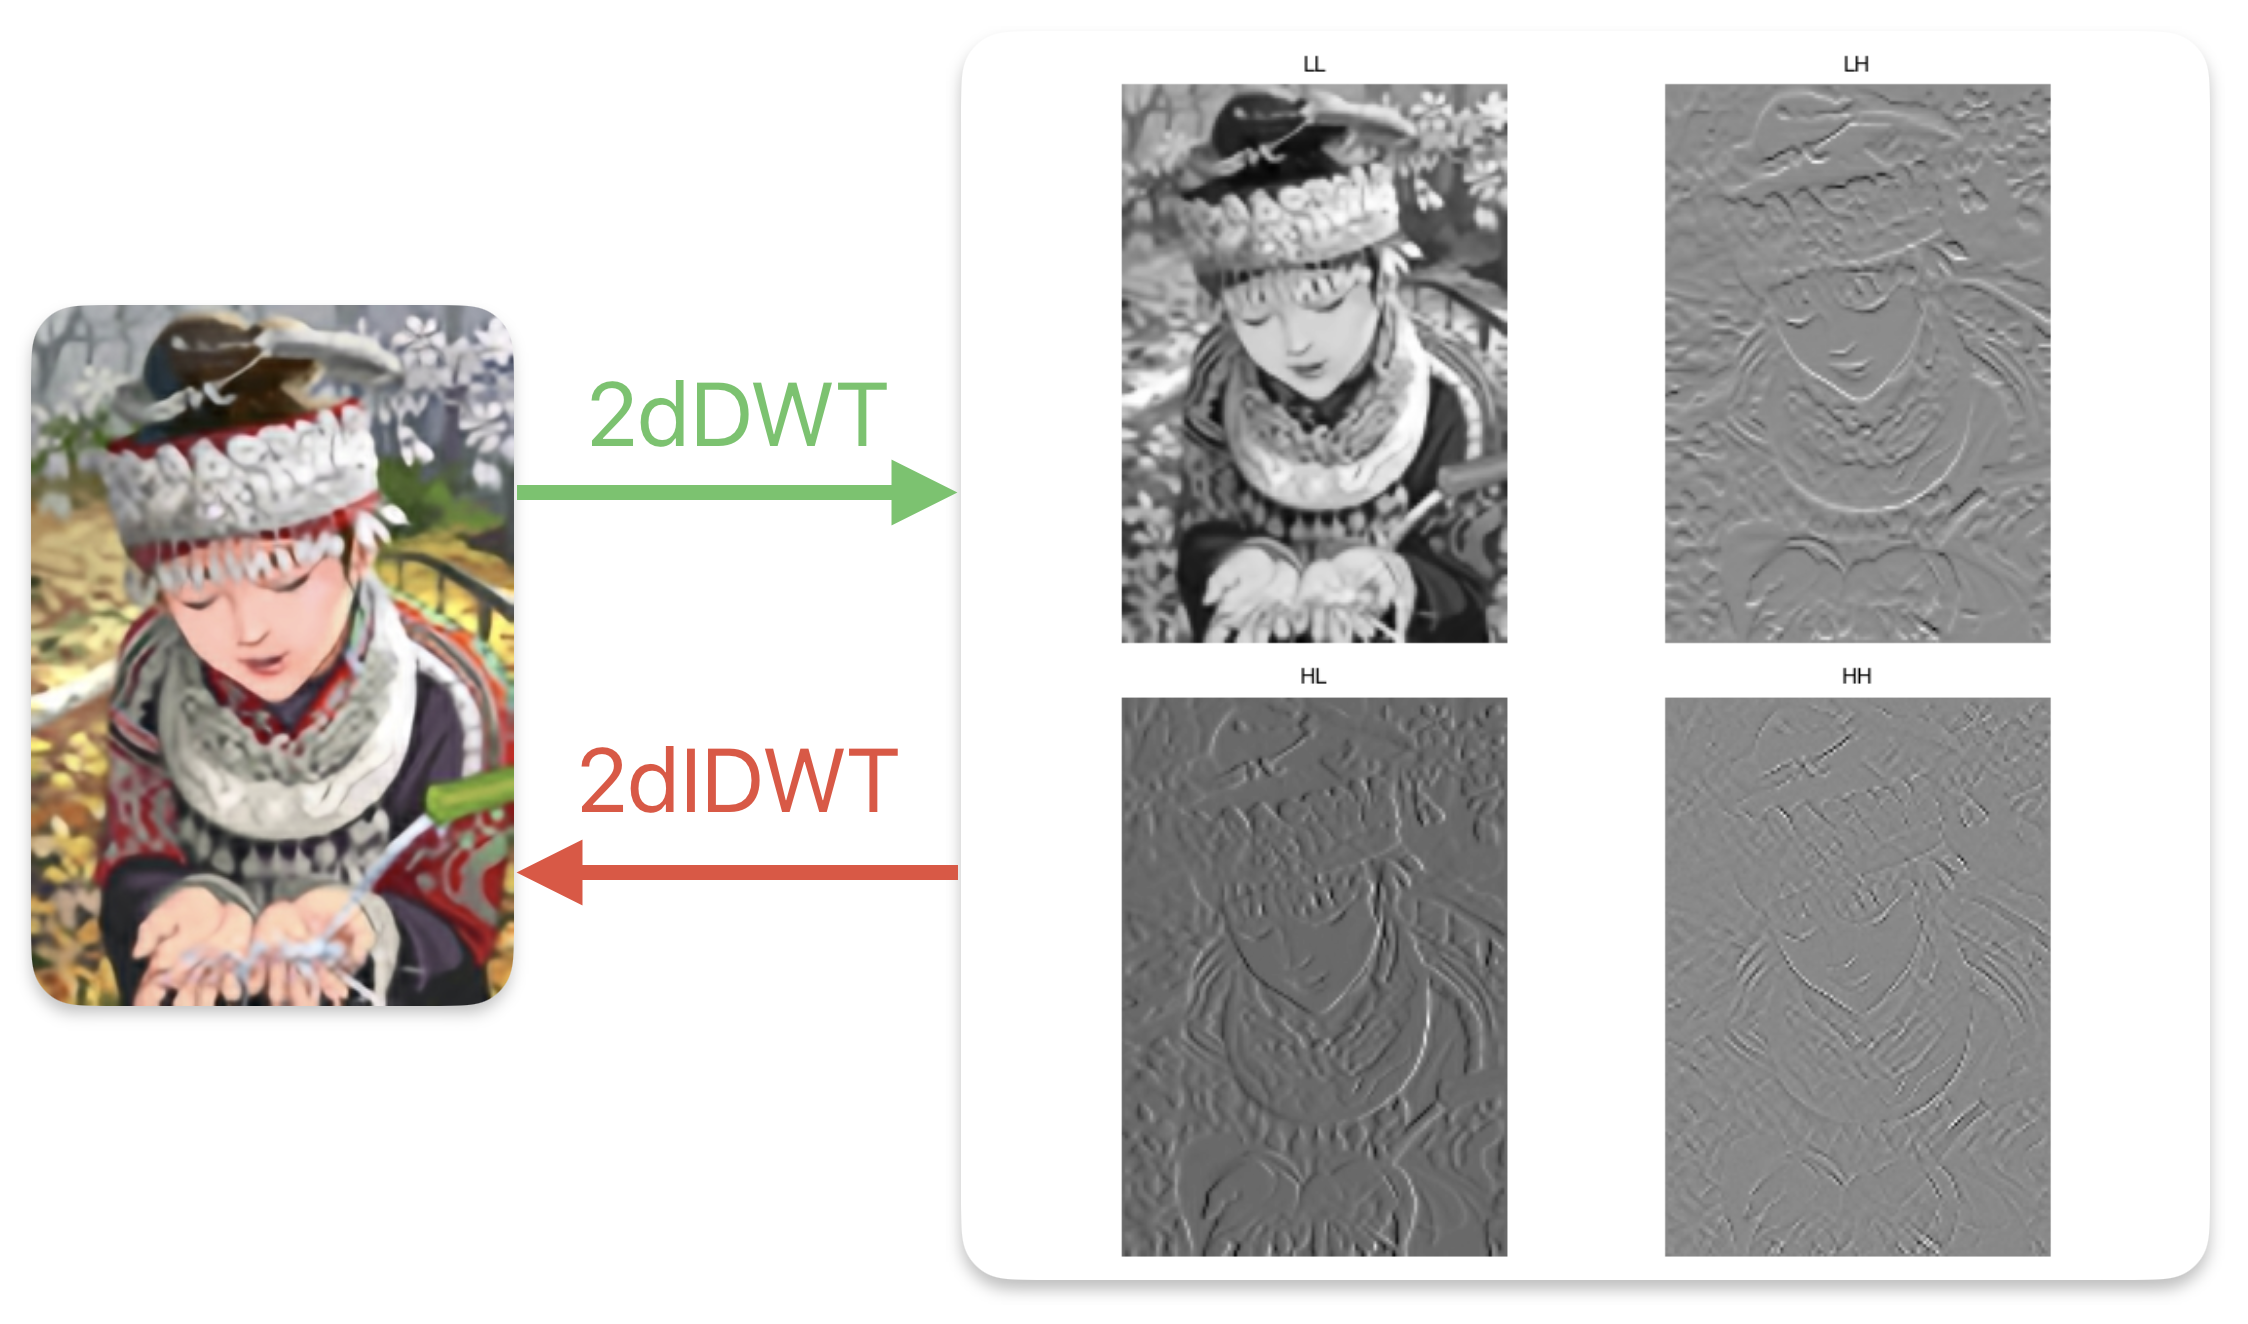
\includegraphics[width=\linewidth]{Rozdziały/03.DWSR/Obrazy/konstrukcja_2dDWT.png}  
        \caption{Proces dekompozycji Dyskretnej Transformacji Falkowej}
        \label{fig:image48}
    \end{minipage}
\end{figure}


Korzystając z falki Haar, współczynniki 2dDWT można zapisać jako:
\begin{equation}
    \left\{\begin{array}{l}
    A=a+b+c+d \\
    B=a-b+c-d \\
    C=a+b-c-d \\
    D=a-b-c+d
    \end{array}\right.
\end{equation}
gdzie: 
\begin{itemize}
    \item $A, B, C, D$ są pikselami w siatce $2 \times  2$ w lewym górnym rogu obrazu HR,
    \item $a$ jest pikselem w lewym górnym rogu obrazu LL,
    \item $b$ jest pikselem w lewym górnym rogu obrazu HL,
    \item $c$ jest pikselem w lewym górnym rogu obrazu LH,
    \item $d$ jest pikselem w lewym górnym rogu obrazu HH.
\end{itemize}

Dlatego przy pomocy transformacji falkowej, problem SR staje się predykcją współczynników falkowych.


\newpage
\subsection*{Struktura sieci}

\begin{figure}[ht]
    \centering
    \begin{minipage}[t]{0.9\linewidth}
        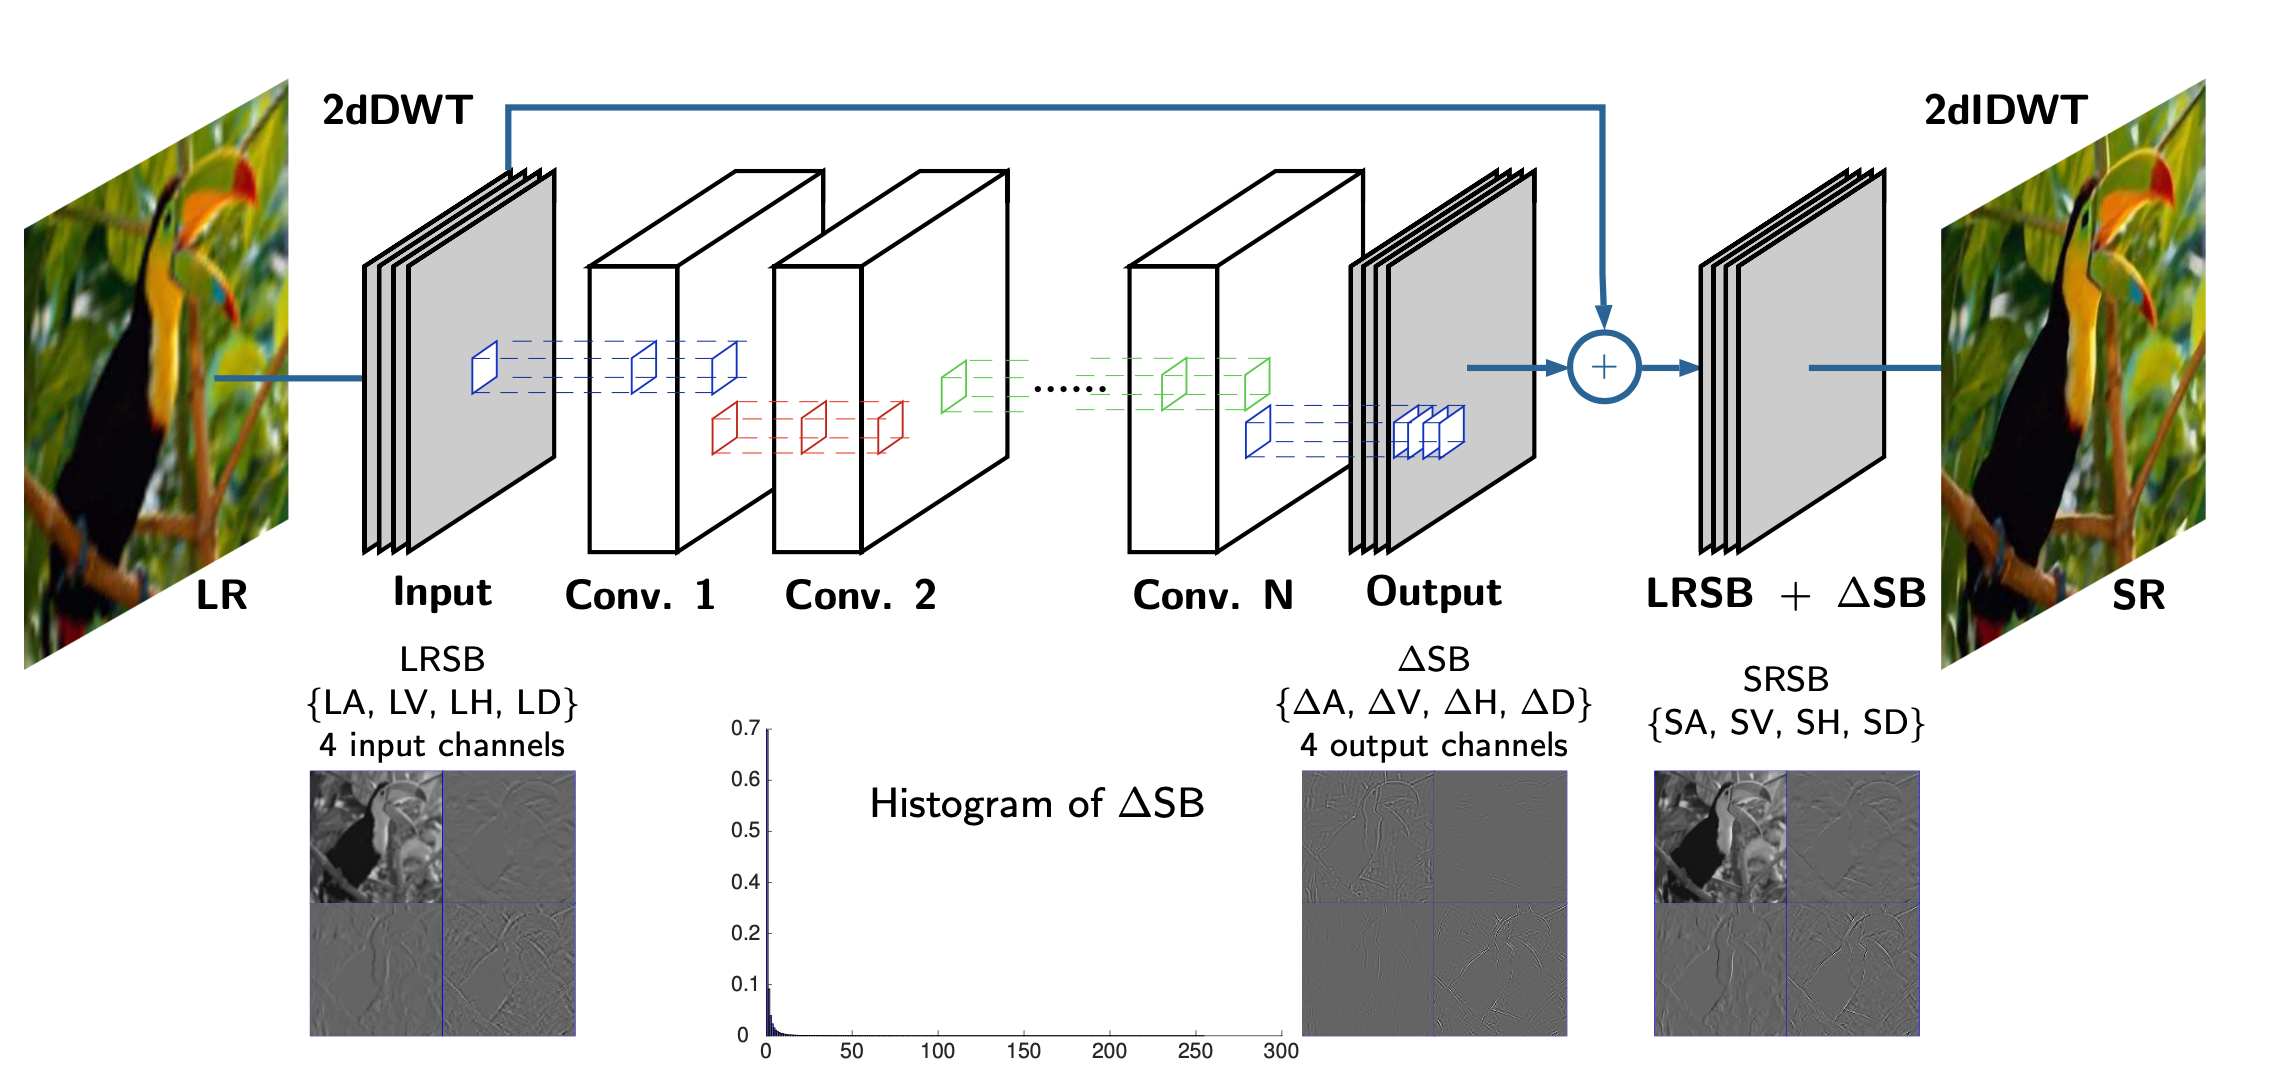
\includegraphics[width=\linewidth]{Rozdziały/03.DWSR/Obrazy/strultura_DWSR.png}  
        \caption{Struktura sieci \textbf{DWSR}}
        \label{fig:image49}
    \end{minipage}
\end{figure}

Strukturę omawianej sieci \cite{guo2017deep} zilustrowano na Rys \ref{fig:image49}. Proponowana sieć ma głęboką strukturę z dwiema warstwami wejściowymi i wyjściowymi z 4 kanałami. Podczas gdy większość metod SR opartych na głębokim uczeniu ma tylko jeden kanał wejściowy i wyjściowy, przedstawiana sieć bierze pod uwagę cztery kanały wejściowe i generuje cztery odpowiadające im kanały na wyjściu. 

W pierwszej warstwie znajdują się 64 filtry o rozmiarze $4 \times  3 \times 3$, a w ostatniej 4 filtry o rozmiarze $64 \times  3 \times 3$. W środkowej części sieci znajduje się N warstw ukrytych o tym samym rozmiarze z $64 \times  3 \times 3 \times 64$ filtrami każda. Dane wyjściowe każdej warstwy, z wyjątkiem warstwy wyjściowej, są podawane do funkcji aktywacji ReLU w celu wygenerowania nieliniowej mapy aktywacji.


\section{Proces treningu}

Obrazy treningowe o niskiej rozdzielczości są powiększane przez interpolację dwusześcienną (omawianą w poprzednim rozdziale). Następnie powiększone obrazy LR są przetwarzane przez 2dDWT z falką Haara w celu uzyskania czterech podpasm LR ($LRSB$), które są oznaczone jako:

\begin{equation}
    L R S B = \left\{ LA, LV, LH, LD \right\} := 2dDWT\left\{LR\right\}, \label{eq:3.2}
\end{equation}

gdzie:
\begin{itemize}
    \item $LA$ - współczynniki LL,
    \item $LV$ - współczynniki HL,
    \item $LH$ - współczynniki LH,
    \item $LD$ - współczynniki HH.
\end{itemize}


\newpage
Transformacja jest aplikowana w podobny sposób do obrazów o wysokiej rozdzielczości, aby uzyskać cztery podpasma HR ($HRSB$), które są oznaczone jako:

\begin{equation}
    H R S B = \left\{ HA, HV, HH, HD \right\} := 2dDWT\left\{HR\right\}, \label{eq:3.3}
\end{equation}

gdzie:
\begin{itemize}
    \item $HA$ - współczynniki LL,
    \item $HV$ - współczynniki HL,
    \item $HH$ - współczynniki LH,
    \item $HD$ - współczynniki HH.
\end{itemize}

Następnie różnicę $\Delta SB$ między $LRSB$ i $HRSB$ można zapisać jako:

\begin{equation}
    \begin{aligned}
    \Delta SB   & ={H R S B} - {L R S B} \\
                & =\{{HA}-{LA}, {HV}-{LV}, {HH}-{LH}, {HD}-{LD}\} \\
                & =\{\Delta {A}, \Delta {V}, \Delta {H}, \Delta {D}\}
    \end{aligned}
    \label{eq:3.4}
\end{equation}

Naszym celem jest wygenerowanie $\Delta SB$ z $LRSB$. Procedura podawania dalej jest oznaczana jako $f(LRSB)$. Koszt wyjścia sieci jest zdefiniowany jako:

\begin{equation}
    \operatorname{cost}=\frac{1}{2}\|\Delta SB-f(LRSB)\|_2^2,
\end{equation}


Wagi i odchylenia zostały oznaczone jako $(\Theta, b)$, następnie problem optymalizacji jest zdefiniowany jako:
\begin{equation}
    (\Theta, {b})=\arg \min _{\Theta, {b}} \frac{1}{2}\|\Delta SB-f(LRSB)\|_2^2+\lambda\|\Theta\|_2^2,
\end{equation}

gdzie $\|\Theta\|_2^2$ jest standardową regulacją rozkładu wag parametru $\lambda$.

Ogólnie rzecz biorąc, sieć jest przygotowana do nauki różnic pomiędzy podpasmami obrazów o wysokiej i niskiej rozdzielczości. W ten sposób sieć uczy się rekonstruować szczegóły obrazu o wysokiej rozdzielczości na podstawie szczegółów obrazu o niskiej rozdzielczości.

\subsubsection*{Generowanie wyników SR}
Aby uzyskać wyniki SR, obrazy wejściowe LR w powiększeniu przez interpolację dwusześcienną są przekształcane przez 2dDWT w celu uzyskania $LRSB$ jako Równanie 3.2.

Następnie $LRSB$ jest przekazywane dalej przez wytrenowaną sieć w celu uzyskania $\Delta SB$. Dodanie $LRSB$ i $\Delta SB$ razem generuje cztery SR wavelet Sub-Bands ($SRSB$) oznaczone jako:

\begin{equation}
    \begin{aligned}
    SRSB    & =\{SA, SV, SH, SD\} \\
            & =LRSB+\Delta SB \\
            & =\{LA+\Delta A, LV+\Delta V, LH+\Delta H, LD+\Delta D\}
\end{aligned}
\end{equation}

W ostatnim etapie 2dIDWT generuje SR obraz jako:

\begin{equation}
    SR=2dIDWT\{SRSB\}
\end{equation}

\subsubsection*{Przygotowanie danych treningowych}


Podczas fazy szkoleniowej wykorzystywanych jest $800$ obrazów szkoleniowych \textbf{NTIRE} \cite{8014883} bez rozszerzenia. Obrazy NTIRE HR 
$\{Y_i\}^{800}_{i=1}$ są próbkowane w dół o współczynnik $c$. 
Obrazy te są powiększane za pomocą interpolacji dwusześciennej o ten sam współczynnik $c$, aby utworzyć obrazy treningowe $LR$ 
$\{X_i\}^{800}_{i=1}$. Należy zauważyć, że obraz $Y_i$ jest przycinany tak, aby jego szerokość i wysokość były wielokrotnością c. Dlatego $X_i$ i $Y_i$ mają ten sam rozmiar, gdzie $Y_i$ reprezentuje obraz treningowy $HR$, zaś $X_i$ reprezentuje odpowiadający mu obraz treningowy $LR$. $X_i$ i $Y_i$ są następnie przycinane do pod-obrazów $41 \times  41$ pikseli z nakładającymi się 10 pikselami do treningu.

Dla każdego pod-obrazu z $X_i$ $LRSB$ jest obliczane jako równanie \ref{eq:3.2}. Dla każdego pod-obrazu z $Y_i$ , $HRSB$ jest obliczany zgodnie z równaniem \ref{eq:3.3}. Następnie resztę $\Delta SB$ jest obliczana zgodnie z równaniem \ref{eq:3.4}.

Zarówno fazy uczenia, jak i testowania \textbf{DWSR} \cite{guo2017deep} wykorzystują tylko informacje o kanale luminancji. W przypadku obrazów kolorowych, kanały $C_r$ i $C_b$ są bezpośrednio powiększane przez interpolację dwusześcienną z obrazów $LR$. Te powiększone kanały chrominancji są łączone z kanałem luminancji $SR$ w celu uzyskania kolorowych wyników $SR$.


\subsubsection*{Ustawienie parametrów treningu}

Sieć została wytrenowana przez \cite{guo2017deep} w następujący sposób.

Podczas procesu uczenia wykorzystywanych było kilka technik. Gradienty są obcinane do $0,01$ za pomocą opcji obcinania normy w pakiecie szkoleniowym. Użyty został optymalizator Adam. Początkowa szybkość uczenia wynosi $0,01$ i zmniejsza się o $25\%$ co 20 epok. 

Regulator wagi jest ustawiony na $1 \times 10^{-3}$, aby zapobiec przeuczeniu. Oprócz warstw wejściowych i wyjściowych, \textbf{DWSR} ma $N = 10$ ukrytych warstw konwolucyjnych o tym samym rozmiarze z filtrem o rozmiarze $64 \times 3 \times 3 \times 64$. Ta konfiguracja skutkuje siecią o relatywnie niewielkiej liczbie parametrów. Schemat uczenia został zaimplementowany za pomocą pakietu TensorFlow z interfejsem interakcji Python 2.7. Użyty został jeden procesor graficzny GTX TITAN X 12 GB zarówno do uczenia, jak i testowania.


\section{Przykłady zastosowań i rezultaty}


Przykładowe wyniki działania algorytmu \textbf{DWSR} przedstawiono na Rys: \ref{fig:image51} \ref{fig:image53}, \ref{fig:image55}. Obrazy pochodzą z repozytorium GitHub, gdzie umieszczony został również algorytm \textbf{DWSR} \cite{guo2017deep}.
\begin{figure}[ht]
    \centering
    \begin{minipage}[t]{0.45\linewidth}
        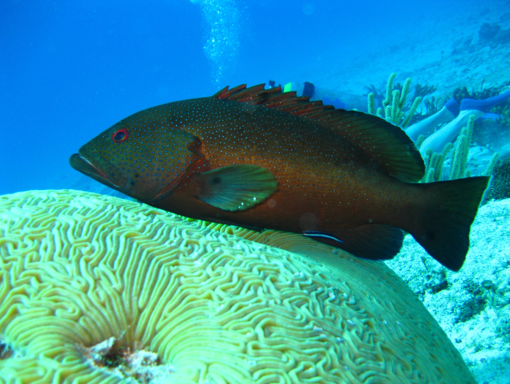
\includegraphics[width=\linewidth]{Rozdziały/03.DWSR/Obrazy/0904x4.png}
        \caption{Obraz wejściowy}
        \label{fig:image50}
    \end{minipage}
    \hspace{0.5cm}
    \begin{minipage}[t]{0.45\linewidth}
        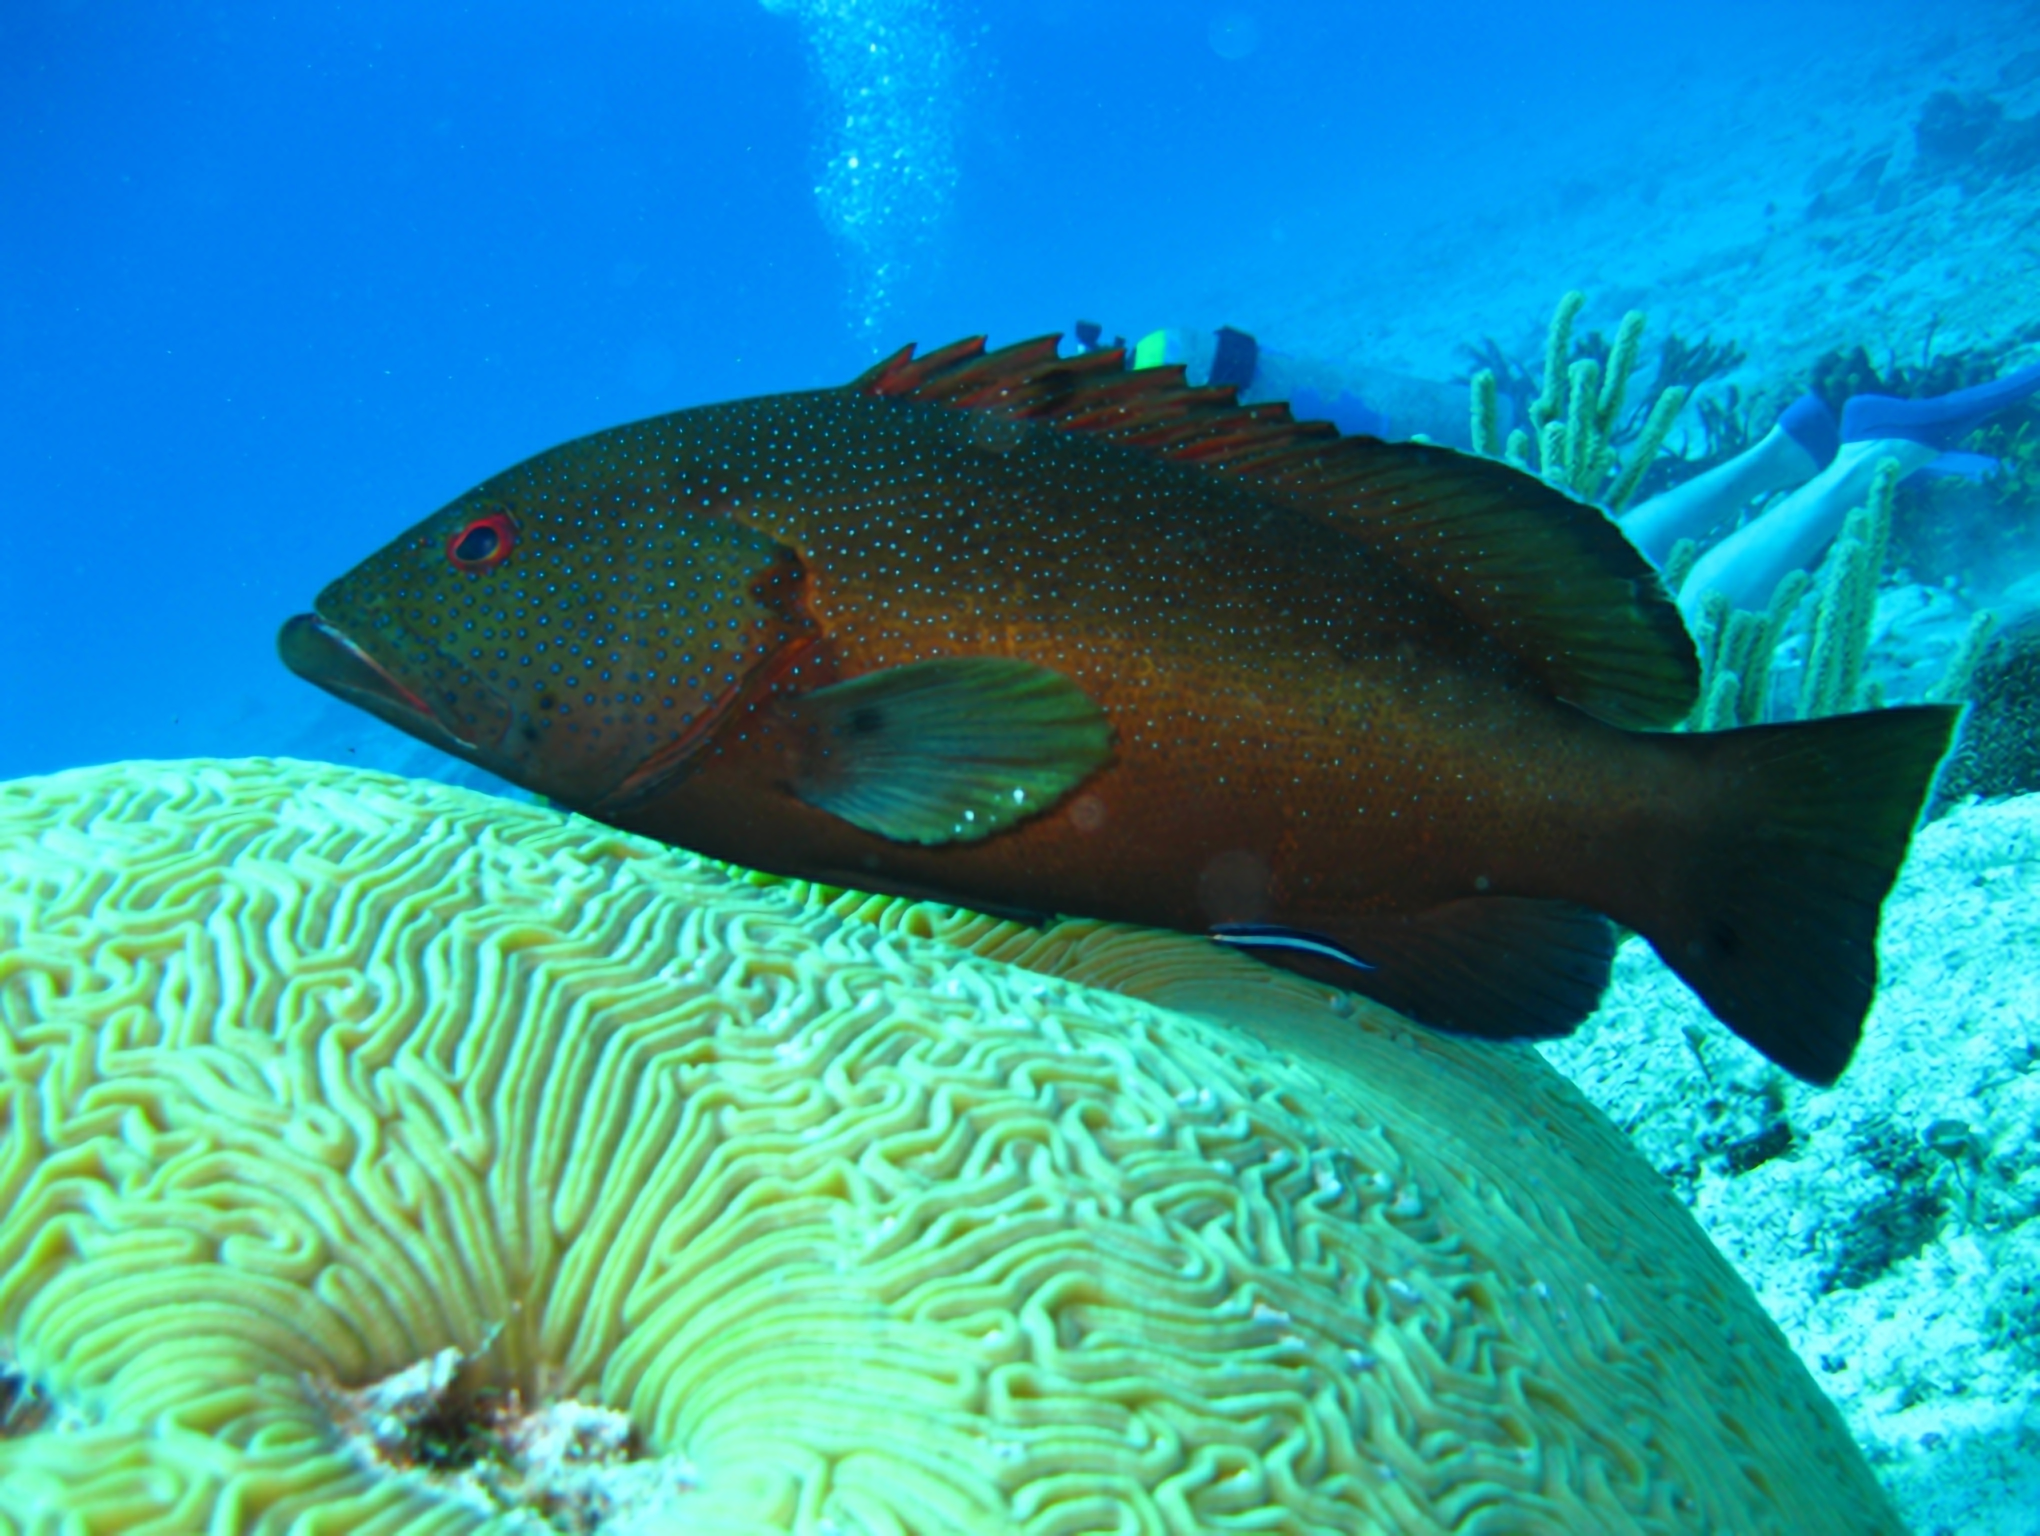
\includegraphics[width=\linewidth]{Rozdziały/03.DWSR/Obrazy/0904x4_DWSRx4.png}
        \caption{Obraz powiększony algorytmem \textbf{DWSR} czterokrotnie}
        \label{fig:image51}
    \end{minipage}
\end{figure}
\begin{figure}[ht]
    \centering
    \begin{minipage}[t]{0.45\linewidth}
        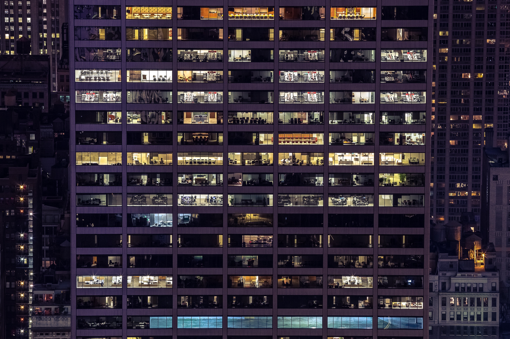
\includegraphics[width=\linewidth]{Rozdziały/03.DWSR/Obrazy/0913x4.png}
        \caption{Obraz wejściowy}
        \label{fig:image52}
    \end{minipage}
    \hspace{0.5cm}
    \begin{minipage}[t]{0.45\linewidth}
        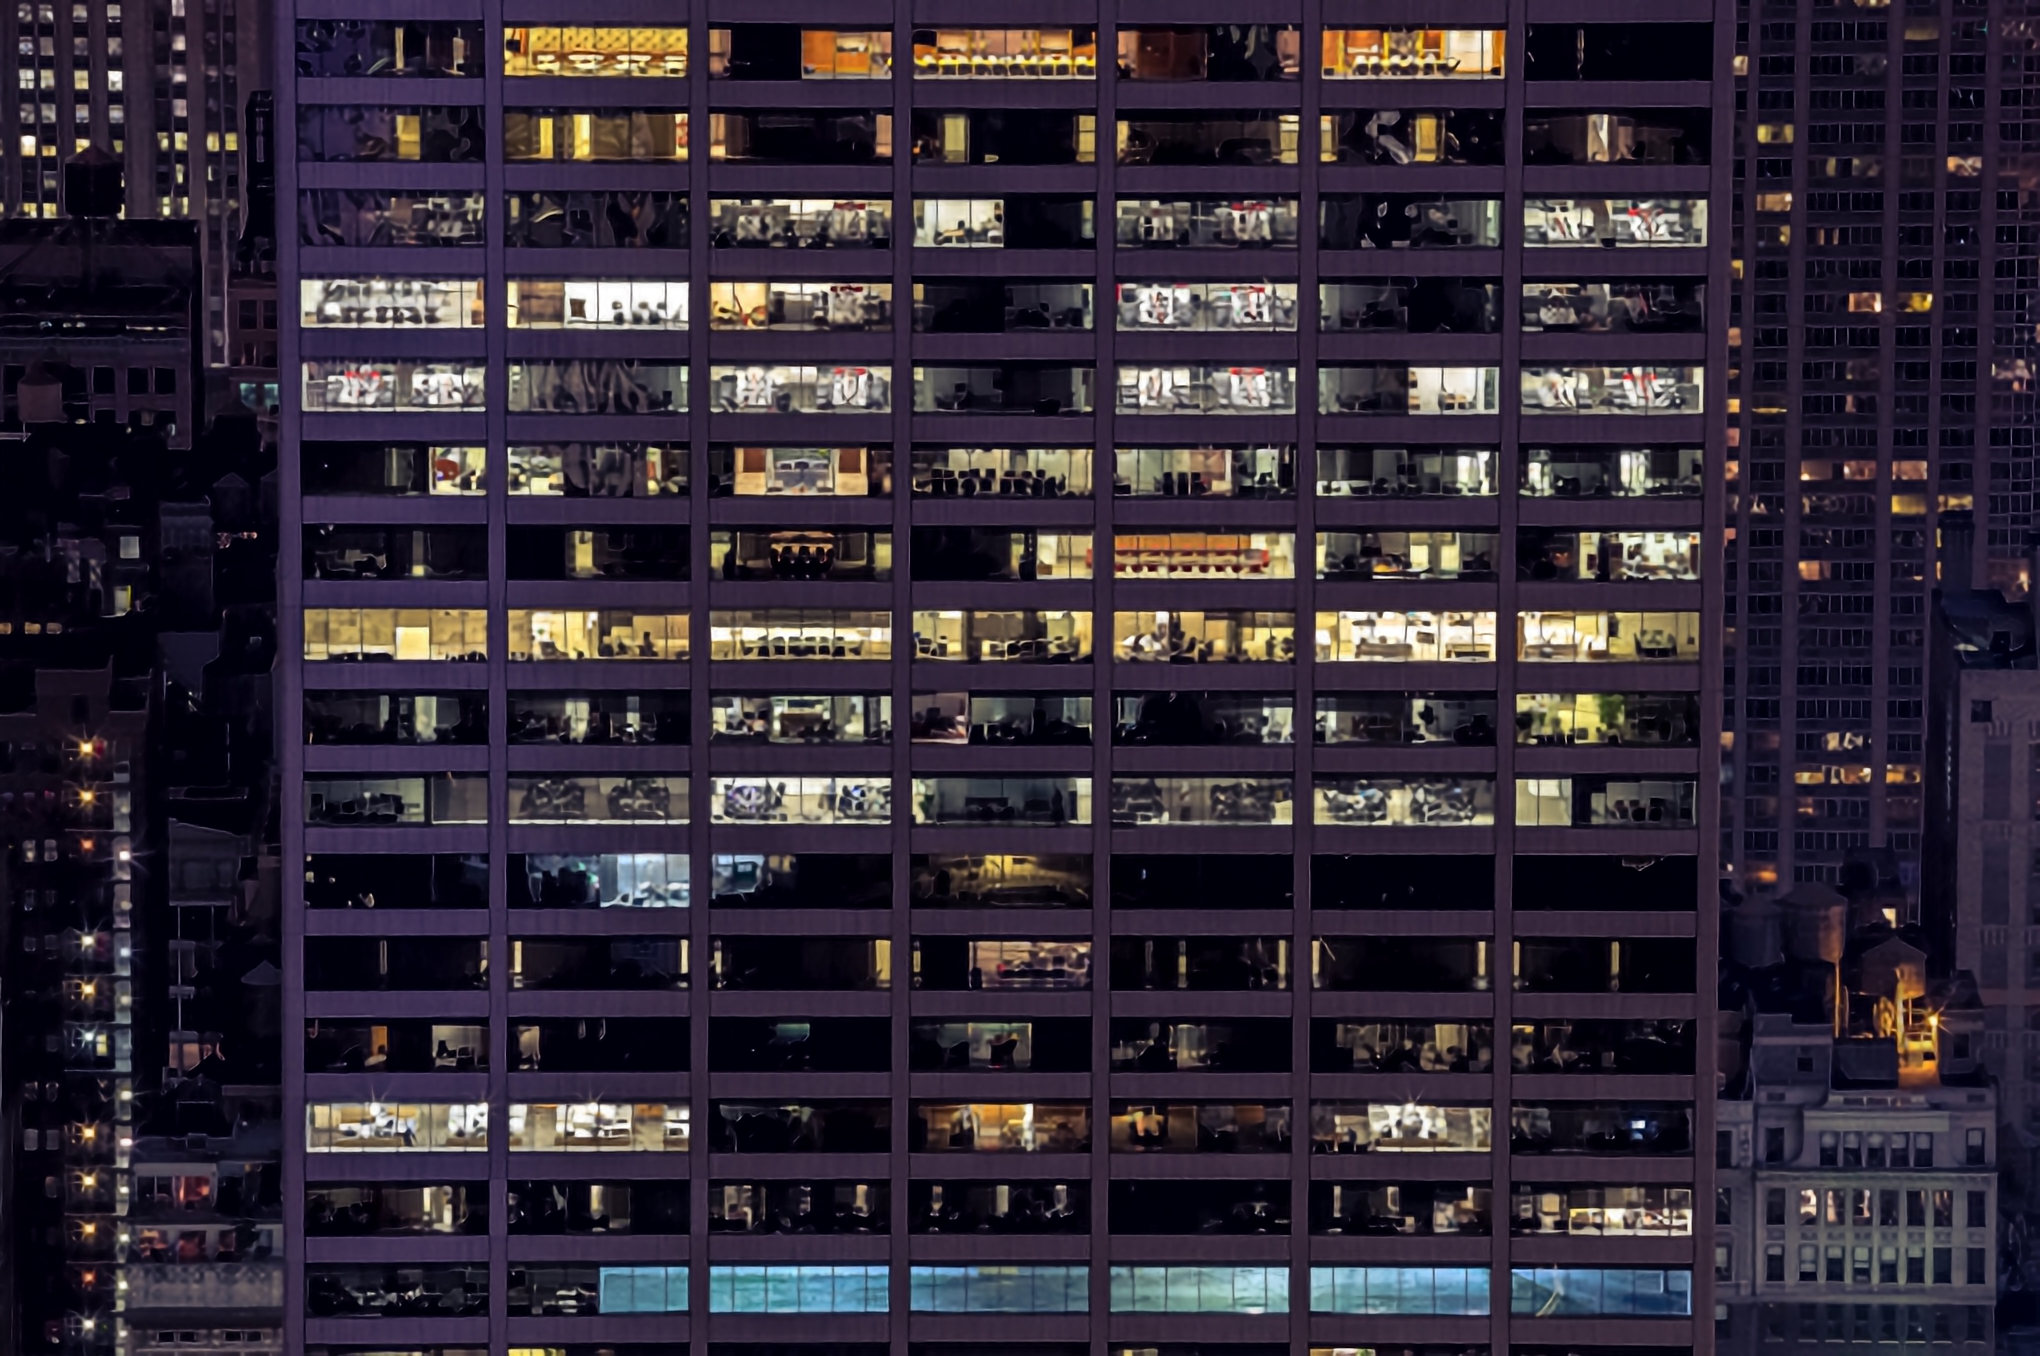
\includegraphics[width=\linewidth]{Rozdziały/03.DWSR/Obrazy/0913x4_DWSRx4.png}
        \caption{Obraz powiększony algorytmem \textbf{DWSR} czterokrotnie}
        \label{fig:image53}
    \end{minipage}
\end{figure}
\begin{figure}[ht]
    \centering
    \begin{minipage}[t]{0.45\linewidth}
        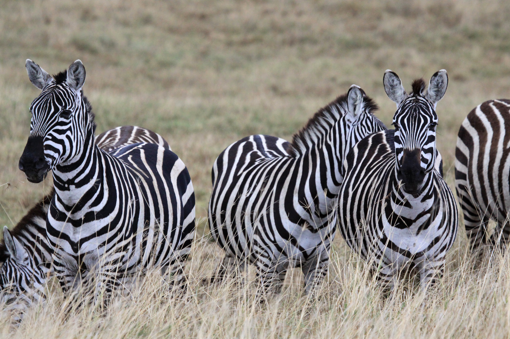
\includegraphics[width=\linewidth]{Rozdziały/03.DWSR/Obrazy/0999x4.png}
        \caption{Obraz wejściowy}
        \label{fig:image54}
    \end{minipage}
    \hspace{0.5cm}
    \begin{minipage}[t]{0.45\linewidth}
        \includegraphics[width=\linewidth]{Rozdziały/03.DWSR/Obrazy/0999x4_DWSRx4.png}
        \caption{Obraz powiększony algorytmem \textbf{DWSR} czterokrotnie}
        \label{fig:image55}
    \end{minipage}
\end{figure}

Ilustracja praktycznych zastosowań DWSR oraz ocena i interpretacja osiągniętych dzięki niemu wyników.
Omawiany algorytm świetnie sobie radzi z rekonstrukcją detali z powtarzających się wzorów, jak na przykład pasy zebry, czy trawa na obrazie \ref{fig:image55}, krawędzie okien na obrazie \ref{fig:image53}, czy tekstura łusek ryby na obrazie \ref{fig:image51}.


Główną zaletą algorytmu \textbf{DWSR} jest szybkość działania, co wynika z niewielkiej ilości parametrów. W porównaniu z innymi metodami SR, \textbf{DWSR} osiąga konkurencyjne lub lepsze wyniki, a jednocześnie jest znacznie oszczędniejsza pod względem liczby parametrów. Dzieje się tak ponieważ falki zapewniają reprezentację obrazu, która naturalnie upraszcza mapowanie, którego należy się nauczyć. 
Dokładniejsza analiza działania algorytmu \textbf{DWSR}, oraz analiza porównawcza z algorytmem \textbf{ESRGAN} została przedstawiona w Rozdziale \ref{chap:porownanie_algorytmow}.